\documentclass[../main.tex]{subfiles}
\graphicspath{{\subfix{../IMAGES/}}}


\begin{document}
\localtableofcontents
\subsection{Introduction}
Deep Learning (DL) $\subset$ Machine Learning (ML) $\subset$ Artificial Intelligence (AI)\\

\begin{itemize}
    \item AI : Any technique that enables machines to mimic human behaviour\\
    \item ML : Ability to learn from data without explicitly being programmed\\
    \item DL : Extract patterns from data using neural networks\\
\end{itemize}

Different types of experience : \begin{itemize}
    \item \underline{Supervised learning} : labels are available\\
    \item \underline{Semi-supervised learning} : some labels are missing\\
    \item \underline{Unsupervised learning} : no labels\\
    \item \underline{Reinforcement learning} : labels are given only as feedback to the program's actions in a dynamic environment\\
    \item \underline{Active learning} : limited set of labels are available and can be interactively selected\\
\end{itemize}

\subsubsection{Notation : data}
$\{ (x^i, y^i)\}_{i=1}^N$ data set consisting of N elements\\
\begin{itemize}
    \item $x^i \in \mathbb{R}^d$ : feature, independent variables, co-variate, explanatory variable\\
    \item $y^i \in \mathbb{R}^n$(continuous) or $y^i \in \{1,2,\dots, k\}$ (discrete set) : target, dependent variable, outcome, response\\
\end{itemize}

\quad \underline{Predictor :}\\
$f:D\rightarrow C$, D the domain and C the co-domain\\
In supervised learning, the data set contains both features and labels. The model learns a function $f$ such that : $f(\text{features}) \simeq \text{label}$\\
We try to learn a predictor $f$, which maps an independent variable $x$ to dependent variable $y$.\\

\subsubsection{Regression vs Classification}
When doing supervised learning, we can either do a regression or classification, it depends on the label's type : \begin{itemize}
    \item label $\in \{1,2,\dots, k\}$ (discrete set) : classification\\
    \item label $\in \mathbb{R}^n$ (continuous set) : regression\\
\end{itemize}
Although, the boundary between regression and classification is not always obvious (possible to transform a regression problem into a classification problem and vice versa).\\

\subsection{Linear Regression}
Model the relationship between two variables by fitting a linear equation to the observed data.\\

It fits a line of slope $w_1$ and of intercept $b$ such that for any data $x^i$, the prediction $\hat{y}^i$ is : \begin{equation}
    \hat{y}^i = wx^i+b
\end{equation}

When there are multiple features, the same principles apply ($x^i \in \mathbb{R}^d)$\\

The model parameters are combined in the \textbf{model parameter vector} such that : \begin{equation}
    \hat{y}^i = b+ w_1x_1 + \dots+w_d x_d^i = w^T x = w^Tx
\end{equation}
Where : \begin{itemize}
    \item $w$ the model's parameter vector : $w = (b, w_1, \dots, w_d)^T \in \mathbb{R}^{d+1}$\\
    \item $x$ is the instance's feature vector : $x=(1,x_1,\dots, x_d)^T \in \mathbb{R}^{d+1}$\\
\end{itemize}

\subsubsection{Loss function}
Given $x\in \mathbb{R}^d$, our model predicts the label $\hat{y} = w^T x$ (true label is $y$).\\

\begin{itemize}
    \item Squared prediction error : $(\hat{y}-y)^2$\\
    \item Mean squared prediction error : $\frac{1}{N} \sum_{i=1}^N (\hat{y}-y)^2$\\
    \item \textbf{Loss function for training} : \begin{equation}
        J(w) = \frac{1}{N} \sum_{i=1}^N (w^Tx^i-y^i)^2
    \end{equation}
\end{itemize}

\quad \underline{Optimizing the loss function :}\\
We search for $w^* \in \mathbb{R}^{d+1}$ such that $J(w^*) \leq J(w)$, $\forall w \in \mathbb{R}^{d+1}$\\

Let $\begin{matrix}
    g:\mathbb{R} \rightarrow \mathbb{R}\\
    J : w\mapsto J(w)\\
\end{matrix}$ if $w^*$ is a minimum, then $\nabla_w J(w^*) = 0$\\

A function $J: \mathbb{R}\mapsto \mathbb{R}$ is convex if $\nabla_w^2 J \geq 0$ $\forall w$\\

For \textbf{convex function}, $w^*$ is a minimum if and only if $\nabla J(w^*) = 0$\\

\quad \underline{Multi-variable :}\\
$J$ is convex if and only if $\nabla^2 J(w) \in \mathbb{R}^{nxn}$ is \textbf{positive semi-definite} ($\lambda \geq 0$).\\
\begin{equation}
    \nabla_w J(w) = \begin{pmatrix}
        \frac{\partial J(w)}{\partial b}\\ \frac{\partial J(w)}{\partial w_1}\\ \dots \\ \frac{\partial J(w)}{\partial w_d}\\
    \end{pmatrix} = \frac{2}{N} \sum_{i=1}^N x^i(w^Tx^i-y^i)
\end{equation}
Where $w\in \mathbb{R}^{d+1} = \begin{pmatrix}
    b\\ w_1 \\ \dots \\ w_d\\
\end{pmatrix}$\\

By putting all x's in the same matrix : $X \in \mathbb{R}^{Nx(d+1)} = \begin{pmatrix}
    1 & x_1^1 & \dots & x_d^1\\
    \dots\\
    1 & x_1^N & \dots & x_d^N\\
\end{pmatrix}$\\

\begin{equation}
    J(w) = \frac{1}{N} (Xw-y)^T(Xw-y)
\end{equation}

Minimizing comes down to (if J is convex) : \begin{equation}
    \begin{gathered}
        \nabla_w J(w) = \frac{2}{N}X^T(Xw-y) = 0 \Leftrightarrow w=(X^TX)^{-1} X^Ty\\
        \frac{\partial^2 J(w)}{\partial w^2} = \frac{2}{N} X^TX\\
    \end{gathered}
\end{equation}

We therefore get : $w^* = (X^TX)^{-1}X^Ty$. Our linear predictor is $f_w(x) = w^{*T}x$\\

Another method : \underline{Gradient descent :}\\

Calculate the gradient of $J(w)$ at the starting point. Iteratively update $w$ by taking steps in the direction of the negative gradient.\\
\begin{equation}
    w^{next} = w-\alpha \nabla_w J(w)
\end{equation}
Where $\alpha$ is the step-size/learning rate.\\

In general, the gradient descent does not converge to the optimal point $w$ unless it is a convex function. \\

\subsubsection{Over-fitting and under-fitting}
The goal of supervised ML is to generalise well on new data based on the patterns learned from known data.

ML can fail in two ways : \begin{itemize}
    \item Over-fitting : fits well on training data but doesn't generalise well to unknown data : model is too complex, it fits noises and errors. Solution : \begin{itemize}
        \item simpler model\\
        \item more training data\\
        \item add a regularisation term\\
    \end{itemize}
    \item Under-fitting : the model doesn't fit well on the training data. The model can't capture the underlying patterns within the data\\
\end{itemize}

\quad \underline{Sensitivity and regularization :}\\
Sensitivity of a predictor : similar data should lead to similar outcome.\\
Less sensitive models tend to not over-fit.\\
Similar data : $x$, $x'$, $\lvert \lvert x-x'\rvert \rvert^2 = (x_1-x_1')^2+ \dots + (x_d+x_d')^2$. If this is small, then x is close/similar to $x'$. \\
$f_w : \mathbb{R}^d\rightarrow \mathbb{R}$ we would like $\lvert f_w(x) - f_w(x)'\rvert$ to be small.\\
With $f_w(x) = b+\omega_1x_1 + \dots + \omega_dx_d$.\\
$\lvert f_w(x) - f_w(x')\rvert = \lvert (\omega_1, \dots, \omega_d) \begin{pmatrix}
    x_1-x_1'\\ \dots \\ x_d-x_d'\\
\end{pmatrix} \rvert \leq \lvert \lvert\omega \rvert \rvert_2 \lvert \lvert x-x'\rvert \rvert_2$\\
$\Rightarrow$ if $\lvert \lvert \omega\rvert \rvert_2$ is small, then $\lvert f_w(x)-f_w(x')\rvert$ will be small when $x$ is similar to $x'$.\\

\quad \underline{Regularised loss function :}\\
\begin{equation}
\begin{gathered}
    J(\omega) = \frac{1}{N} \sum_{i=1}^N (\omega^T x^i-y^i)^2+ \lambda(\omega_1^2+\dots + \omega_d^2) = \frac{1}{N} (X\omega-y)^T(X\omega -y) + \omega^T \lambda \omega\\
    \nabla J(\omega) = \frac{2}{N} X^T(X\omega-y)+2\lambda \omega\\
    \end{gathered}
\end{equation}
Where $\lambda$ is a parameter.

\subsection{Logistic Regression}
We can use regression for a classification problem by adapting the outputs.\\

The goal of logistic regression is to find a separation.\\
\begin{equation}
    y = \{ \text{"type 1", "type 2"} \} = \{0,1\}
\end{equation}

\quad \underline{Loss function :}\\
$\{ (x_i, y_i)\}_{i=1}^N$, $y^i \in \{0,1\}$\\
$z = b+w_ix_i + \dots + w_dx_d$\\
Classifier : $\begin{cases}
    z\geq 0 & \hat{y}=1\\
    z \leq 0 & \hat{y}=0\\
\end{cases}$
\begin{equation}
    J(w) = \frac{1}{N} \sum_{i=1}^N [(1-y^i)\log(1+e^{z_i}) + y^i \log(1+e^{-z_i})]
\end{equation}

How to fit the parameters $w$ and $b$ : $\min_{w,b}J(w,b)$\\

\subsubsection{Confusion matrix}
\begin{enumerate}
    \item $y=0$, $\hat{y}=0$ : true negative, $C_{tn}$ number of true negative\\
    \item $y=0$, $\hat{y}=1$ : false positive $C_{fp}$\\
    \item $y=1$, $\hat{y}=0$ : false negative $C_{fn}$\\
    \item $y=1$, $\hat{y}=1$ : true positive $C_{tp}$\\
\end{enumerate}

\begin{table}[hbt!]
    \centering
    \begin{tabular}{c|c|c|}
    
    &\multicolumn{2}{c}{true label}\\
    \hline
    prediction & $C_{tn}$ & $C_{fn}$ \\ \cline{2-3}
     & $C_{fp}$ & $C_{tp}$\\ \cline{2-3}
    \end{tabular}
\end{table}

\begin{itemize}
    \item Number of data points : $N = C_{tn}+C_{fn}+C_{fp}+C_{tp}$\\
    \item Error rate : $\frac{C_{fn}+C_{fp}}{N}$\\
    \item Accuracy : $\frac{C_{tn}+C_{tp}}{N}$\\
    \item Recall : fraction of positives that are correctly classified $\frac{C_{tp}}{C_{tp}+C_{fn}}$\\
\end{itemize}

\subsection{Ethics of AI}
Ethics is an investigation about values and how these values are implemented in different tools/practices.\\

\subsubsection{Ethics in the technology}
\begin{itemize}
    \item Data ethics\\
    \item Algorithmic ethics\\
    \item Interface/design ethics\\
    \item Sustainability\\
    \item Integration in decision-making process\\
\end{itemize}

\subsubsection{Social Justice}
\begin{itemize}
    \item Impact on labor market\\
    \item Impact on social interactions\\
    \item Impact on inequality\\
    \item Access to technology\\
\end{itemize}

\subsubsection{Impact on framing/narratives}
\begin{itemize}
    \item The competition or instrument relationship between human beings and machines\\
    \item The specificity of human beings\\
    \item The meaning and purpose of human life\\
\end{itemize}

\subsection{Feature engineering}

Setting hyper-parameters : \begin{enumerate}
    \item Split data into train and test, choose hyper-parameters that work best on test data : inconvenient we have no idea how the algorithm will perform on new data\\
    \item Split data into \textbf{train}, \textbf{validation} and \textbf{test}, choose hyper-parameters on validation and evaluate on test\\
    \item cross-validation : split data into \textbf{folds}, try each fold as validation and average the results (useful for small datasets)\\
\end{enumerate}

\subsubsection{Probabilistic interpretation of logistic regression}
Consider the regression $z^i = w^Tx^i+b$ and the \textbf{logistic function} : \\
$\hat{y}^i = \frac{1}{1+e^{-(w^Tx^i+b)}} = logit(z) = \sigma(z)$\\
Where : \begin{itemize}
    \item $\hat{y}^i$ the estimated probability that $y=1$ on input $x^i$\\
\end{itemize}

\quad \underline{Cross entropy of a distribution relative to another :}\\
Cross entropy of q related to p is defined as : $-\sum_{i=1}^n p(i)\log(q(i))$\\
The cross entropy of our predicted distribution of label $\{0,1\}$ related to true distribution is : \\
$-[p(y=1| x^i)\log(\hat{y}^i) + p(y=0|x^i) \log(1-\hat{y}^i)] = N L(\omega)$\\

The cross entropy between the true distribution and the estimated distribution is the logistic loss.\\

\subsubsection{Multi-nomial logistic regression}

Extend the logistic function to the multi-class setting by defining the soft-max function : \begin{equation}
    \text{soft-max}(z) = (\frac{\exp(z_1)}{\sum_{j=1}^k \exp(z_j)},\dots, \frac{\exp(z_k)}{\sum_{j=1}^k \exp(z_j)})
\end{equation}
Each component will be in the interval (0,1) and they will add up to 1.\\

\underline{Cross-entropy Loss :}\begin{equation}
    J(w,b) = -\frac{1}{N} \sum_{i=1}^N \sum_{c=1}^k \mathbf{1}\{y^i=c\} \log(\frac{\exp(z^i_c)}{\sum_{j=1}^K\exp(z^i_j)})
\end{equation}

\quad \underline{Performance metric :}\\
\begin{itemize}
    \item Confusion matrix : (assume 3 classes for representation) \begin{table}[hbt!]
        \centering
        \begin{tabular}{|c||c|c|c|}
        \hline
         & class 1 & class 2 & class 3\\    \hline     \hline
        class 1 & $C_{1,1}$ & $C_{1,2}$ & $C_{1,3}$ \\ \hline
        class 2 & $C_{2,1}$ & $C_{2,2}$ & $C_{2,3}$ \\ \hline
        class 3 & $C_{3,1}$ & $C_{3,2}$ & $C_{3,3}$\\ \hline
        \end{tabular}
        \caption{True label vs. Predicted label}
    \end{table}
    Where the $C_{ij}$ are numbers of class j data points that are predicted as class i\\
    \item Accuracy : $\frac{IC}{N} = \frac{C_{11} + C_{22}+C_{33}}{N}$\\
    \item Error rate : $1-A$\\
\end{itemize}


\subsubsection{Input representation}
\begin{center}
    Feature engineering means transforming \textbf{raw data} into a \textbf{feature vector} that represents the underlying data well
\end{center}

Different types of features : \begin{itemize}
    \item Numerical/continuous (height, $\dots$)\\
    \item Ordinal (like, somewhat like, dislike)\\
    \item Categorical (color, $\dots$)\\
\end{itemize}

\quad \underline{Preprocessing :} the process of transforming raw feature vectors into a representation that is more suitable for ML algorithms.\\

\quad \underline{Numerical features :}\\
We can have different approaches : \begin{itemize}
    \item If the value of a component is positive and ranges over a wide scale : take the log of every value\\
    \item Binning/discretization : partition continuous features into discrete values \begin{itemize}
        \item Uniform : all bins have identical widths\\
        \item Quantile : all bins have the same number of points\\
        \item Clustered : a clustering algorithm is used to separate values\\
    \end{itemize}
\end{itemize}

\quad \underline{Ordinal features :}\\
Ordinal variables are a \textbf{finite set} of discrete values with a \textbf{clear ordering} between them.\\
Integer encoding : map values to integers ranging from 1 to n.\\

\quad \underline{Categorical features :}\\
Categorical variables are a \textbf{finite set} of discrete values with \textbf{no intrinsic ordering} between them.\\
We use here a \textbf{one-hot encoding} : each category is represented by a binary variable (eg : $\begin{pmatrix}
    \text{cat}\\ \text{dog}\\
\end{pmatrix} \rightarrow \{ \begin{pmatrix}
    1 \\ 0 \\
\end{pmatrix}, \begin{pmatrix}
    0\\ 1\\
\end{pmatrix}\}$)\\

\subsubsection{Missing values}
Raw data isn't clean and we might find some missing values. Many ML algorithms cannot work with missing values.\\

How to handle missing data : \begin{itemize}
    \item Deletion : if a few features have missing values, delete them\\
    \item Imputation : replace missing values by another one \begin{itemize}
        \item For numerical data : \begin{itemize}
            \item Constant imputation : impute with constant value different from all other values\\
            \item Mean imputation : impute with mean\\
            \item KNN imputation : impute with mean of k nearest neighbors\\
        \end{itemize}
        \item For ordinal data : \begin{itemize}
            \item Constant imputation : impute with constant value different from all other values\\
            \item Median imputation : impute with median\\
            \item KNN imputation : impute with median of k nearest neighbors\\
        \end{itemize}
        \item For categorical data : \begin{itemize}
            \item Add new category : corresponding to "missing data"\\
            \item Mode imputation : impute with the mode of the feature (most common category)\\
            \item KNN imputation : impute with mode of k nearest neighbors\\
        \end{itemize}
    \end{itemize}
\end{itemize}

\subsubsection{Feature expansion}
If a data set is not linearly separable, we can add a synthetic feature that combine the original ones. Doing so makes the data linearly separable.\\

Feature expansion is the process of creating derived features from the input data. It adds complexity, reduces under-fitting and can improve performance.\\
Popular feature expansion : \begin{itemize}
    \item Feature crosses : multiply features together\\
    \item Binning : transform a numerical feature into categorical/ordinal features\\
    \item Applying a non-linear function to each feature\\
\end{itemize}

Polynomial feature expansion with interaction generates a new feature vector consisting of all polynomial combinations of features with degree less than or equal to a given degree.\\


\subsection{Data statistics}
The probabilistic distribution is given by : \\
$S = \{(s_1,\dots, s_n)\}$\\
$P : S\rightarrow \mathbb{R} \sum_{i=1}^n p(s_i)=1$\\

\begin{itemize}
    \item Data $\{x_i\}_{i=1}^n \in \mathbb{R}$\\
    \item Mean (average value) : $\mu = \frac{1}{N} \sum_{i=1}^n x_i$\\
    \item Variance (measures how far values are from mean) : $\frac{1}{N} \sum_{i=1}^n (x_i-\mu)^2 = \sigma^2$\\
    \item Standard deviation $\sigma$\\
    \item k-th q-quantile (data needs to be ordered from lowest to highest value) : index of data as $I = \frac{Nk}{q}$, $\begin{cases}
        \text{if I is an integer, return }x_I \text{ or } x_{I+1}\\
        \text{if I is not an integer, round up to nearest integer, return } x_I\\
    \end{cases}$
    \item Mode (most occurring value)\\
    \item corr$(x_j, x_j') = \frac{cov(x_j, x_j')}{\sigma_j \sigma_j'}$\\
\end{itemize}

\quad \underline{Data normalization :}\\
Also feature scaling. Two different kind : \begin{itemize}
    \item Min-max scaling : scale each dimension of data to the range [0,1] \begin{equation}
        x_{norm} = \frac{x-\min(x)}{\max(x)-\min(x)}
    \end{equation}
    \item Z-score normalization/standardization : set mean of each dimension to 0 and standard deviation to 1 \begin{equation}
        x_{norm} = \frac{x-\mu_x}{\sigma_x}
    \end{equation}
\end{itemize}

\subsection{Naive Bayes classifier}
It is a probabilistic classifier.\\

\quad \underline{Joint distribution :}\\
Two events are independent if \begin{equation}
    P(A\cap B) = P(A)P(B)
\end{equation}

\quad \underline{Conditional distribution :}\\
Conditional distribution is a probability distribution conditioned on an event : $P(A=i \lvert B=b) \Rightarrow \sum_{i=1}^n P(A=i \lvert B=b) = 1$\\

A and B are independent if  : \begin{equation}
    P(A=i \lvert B=b) = P(A=i)
\end{equation}

Or even, A and B are conditionally independent given C if $P(A\cap B\lvert C) = P(A\lvert C) P(B\lvert C)$\\

Marginal distribution : $P(A) = \sum P(A \lvert B=b)$\\

\quad \underline{Bayes theorem :}\\
\begin{equation}
    P(B\lvert A) = \frac{P(A\cap B)P(B)}{P(A)}
\end{equation}

In our case, we have a classifier $c\in \{0,1\}$ :\\
\begin{equation}
    \begin{cases}
        P(y=0\lvert x) > P(y=1\lvert x) & \text{ predict class 0}\\
        \text{else } & 1\\
    \end{cases}
\end{equation}
Therefore, we need to compare : $P(x\lvert y=0) P(y=0) > P(x\lvert y=1) P(y=1)$\\

Or equivalently : \\
\begin{equation}
    P(y=1\lvert x) = \frac{\Pi_{j=1}^d P(x_j \lvert y=c)P(y=c)}{P(x)}
\end{equation}

$P(y=1\lvert x)> P(y=0\lvert x) \Rightarrow \Pi_{i=1}^d P(x_j \lvert y=1) P(y=1) > \Pi_{j=1} P(x_j \lvert y=0)P(y=0)$\\

\subsubsection{Continuous features}
\begin{equation}
    P(y=c\lvert x) = \frac{f_{x\lvert y=c}(x) P(y=c)}{f_x(x)}
\end{equation}
\begin{itemize}
    \item $Pr(x=v) = 0$, $\forall v \in \mathbb{R}^d$\\
    \item $Pr(x\in D) = \int_D f_x(x)dx$\\
    \item $\int_{\mathbb{R}^d} f_x(x)dx =1$\\
    \item $f_x(x) \geq 0$, $\forall x \in \mathbb{R}^d$\\
\end{itemize}

$f_{x\lvert y=c}(x)$ : conditional probability density of $x$ given class $c$\\
The Naive Bayes assumption is : $f_{x\lvert y=c}(x) = \Pi_{j=1}^df_{x_j \lvert y=c}(x_j)$ : features conditionally independent given.\\

Assume that the generative model for each feature follows a \textbf{Gaussian distribution}. \\
\begin{equation}
    f_{x_j\lvert y=c} (x_j) = \frac{1}{\sqrt{2\pi \sigma_{j,c}^2}}e^{-\frac{1}{2}(\frac{x-\mu_{j,c}}{\sigma_{j,c}})^2} = N(\mu_{j,c}, \sigma_{j,c}^2)
\end{equation}

\begin{itemize}
    \item $\mu_{j,c} = \frac{1}{\lvert I_c\rvert} \sum_{i\in I_c} x_j^i$ : mean of data of feature given class label $c$, $I_c$ has the indices of data corresponding to class $c$\\
    \item $\sigma_{j,c}^2 = \sum_{i\in I_c} \frac{(x_j^i-\mu_{j,c})^2}{\lvert I_c\rvert}$ : variance\\
\end{itemize}

\subsection{k-Nearest Neighbour}
Use dataset to produce useful predictions on never-before-seen data. \\
KNN (K-Nearest Neighbors) : algorithm assumes that data points of similar classes exist in close proximity\\

It classifies an unknown data point according to the category of its K nearest neighbors.\\

\subsubsection{Measure distance}
Let $x^1$, $x^2 \in \mathbb{R}^d$\\
Minkowski distance : \begin{equation}
    D(x^1,x^2) = (\sum_{j=1}^d(x_j^1-x_j^2)^p)^{\frac{1}{p}}
\end{equation}

\begin{itemize}
    \item $p=1$ Manhattan distance (L1)\\
    \item $p=2$ Euclidean distance (L2)\\
\end{itemize}

Features might have different scales. Distance metric gives more importance to the feature with largest scale.\\

\subsubsection{Implementation}
\begin{itemize}
    \item Initialize k\\
    \item For every unknown data point calculate the distance with the unknown data point\\
    \item Pick the k nearest known data points from the unknown data point\\
    \item Get the labels of the selected k entries\\
    \item Return the mode (majority vote) of the k labels\\
\end{itemize}

\subsubsection{Hyper-parameters}
What is the best value of k and the best distance? We set them rather than learn.\\


\begin{minipage}{.49\textwidth}
    Advantages : \begin{itemize}
        \item Easy to implement \\
        \item No training required \\
        \item New data can be added\\
    \end{itemize}
\end{minipage}
\vline
\begin{minipage}{.49\textwidth}
    Disadvantages : \begin{itemize}
        \item It does not work well in high dimensions\\
        \item Sensitive to noisy data\\
        \item Requires high memory\\
        \item Prediction stage is slow\\
    \end{itemize}
\end{minipage}

\subsection{Dimensionality reduction}
$x^i \in \mathbb{R}^d$ but d can be very large.\\
We want to find a smaller set of new features that explain our sample.\\

\subsubsection{Principal Component Analysis (PCA)}
Find the best linear combination of features to create new features that explain our samples.\\

Let $\theta_1, \dots, \theta_r \in \mathbb{R}^d$.\\
A linear combination of $\{\theta_j\}_{j=1}^r$ is given by $a_1\theta_1 + \dots + a_r \theta_r$, $a_i \in \mathbb{R}$\\

$S=\{\sum_{j=1}^r a_j \theta_j \lvert a_j \in \mathbb{R}, j=1,\dots, r\}$ is a \textbf{subspace} spanned by $\{\theta_j\}_{j=1}^r$\\

We define a distance of a point to a subspace as : \begin{equation}
\begin{gathered}
    dist(x,S) = \min_a \lvert \lvert x-\theta a\rvert \rvert_2 \Rightarrow a^* = argmin\lvert \lvert x-\theta a\rvert \rvert_2 = (\theta^T\theta)^{-1}\theta^Tx\\
    dist(x,S) = \lvert \lvert x-\theta(\theta^T\theta)^{-1}\theta^Tx\rvert \rvert_2\\
    \end{gathered}
\end{equation}

Where $\hat{x}$ is the projection of $x$ onto $S$ : $\hat{x} = \theta(\theta^T\theta)^{-1}\theta^Tx$\\

The objective function in PCA is to minimize : \begin{equation}
    \frac{1}{N} \sum_{i=1}^N dist(x_i,S) = \frac{1}{N}\sum_{i=1}^N \lvert \lvert x^i-\hat{x}^i\rvert \rvert_2
\end{equation}

Althought, we first need to \textbf{standardize} the data : let $X \in \mathbb{R}^{Nxd}$\\
$X = \begin{pmatrix}
    X_1^1 & X_2^1 & \dots & X_d^1\\
    \dots & \dots & \dots & \dots\\
    X_1^N & X_2^N & \dots X_d^N\\
\end{pmatrix}$

\textbf{Frobenius norm of a matrix :} \begin{equation}
    \lvert \lvert X\rvert \rvert_F = \sqrt{\text{Trace}(X^TX)}
\end{equation}

Then, the PCA objective function is : \begin{equation}
    \min_\theta \frac{1}{N} \lvert \lvert X-X\theta^T\theta\rvert \rvert_F^2, \quad \theta \in \mathbb{R}^{dxr}
\end{equation}

We can now decompose the matrix $\mathbf{C = X^TX} \in \mathbb{R}^{dxd}$\\
C is symmetric. \\
For any symmetric matrix, there exists an eigenvalue/eigenvector decomposition $C = VDV^T$.\\
With $D = \begin{pmatrix}
    \lambda_1 & \dots & 0\\
    0 & \dots & 0\\
    0 & \dots & \lambda_d\\
\end{pmatrix}$ a diagonal matrix with $\lambda_i \in \mathbb{R}$ the eigenvalues of C\\
$V\in \mathbb{R}^{dxd} = (V_1,\dots, V_d)$ a matrix filled with the eigenvectors of C and $V^TV = I$\\

Assume $\lambda_1 \geq \dots \geq \lambda_d$ then $\theta_1 = v_1 \dots \theta_r = v_r$\\
Subspace S is the span of the first r eigenvectors of $X^TX$. $v_i$ are called \textbf{principal component of the data}. \\
New features are therefore : $A = X\theta$\\
$\hat{X} = X\theta\theta^T$ is the reconstruction of X based on this new subspace.\\

How to find the first set of value? \\
\subsubsection{TFIDF}
Term-frequency and inverse document frequency\\
Used to distinguish texts.\\

\begin{itemize}
    \item Term frequency of word j in document $u_i$ : $f_{term}(u_i,j) = \frac{\text{number of times word j appears in }u_i}{\text{number of words in document }u_i}$\\
    \item Document frequency of word j : $f_{doc}(j) = \frac{\text{number of times word j appear in all documents}}{\text{number of documents}}$\\
\end{itemize}

The TFIDF for each word is : $x_j^i = f_{term}(u_i,j) \ln(\frac{1}{f_{doc}(j)})$\\

There are several other techniques for dimensionality reduction : \begin{itemize}
    \item Linear discriminant analysis (LDA)\\
    \item Generalized discriminant analysis (GDA)\\
    \item T-distributed Stochastic Neighbor Embedding (t-SNE)\\
    \item Auto-encoders\\
\end{itemize}

\subsubsection{Auto-encoders}
It is a type of neural network often used for dimensionality reduction. They are trained in an unsupervised manner by minimizing the reconstruction error/loss $\sum_{i=1}^NL(x^i,\hat{x}^i)$\\
$\hat{x}^i$ is a non-linear combination of original feature.\\

\subsection{Clustering}

The goal is to group data points as a first step to understand the data set.\\
\textbf{k-means :} Group points based on their proximity.\\

Main idea : \begin{itemize}
    \item identify k cluster of data points given N samples\\
    \item find prototype (representative) points $\mu_1, \dots, \mu_k$ representing the center of each cluster\\
\end{itemize}

Let $\{\mu_1,\dots, \mu_k\} \subseteq \mathbb{R}^d$ be our cluster centers.\\
Determine the cluster of a single point $x_i$ with $\min_{j=1,\dots, k} \lvert \lvert x^i-\mu_j \rvert \rvert_2^2$.\\
Determine the cluster centers to minimize the distance of each point to its assigned cluster : k-means tries to find $\min_{\mu_1,\dots, \mu_k} \sum_{i=1}^N \min_{j=1,\dots,k} \lvert \lvert x^i-\mu_j\rvert\rvert_2^2$\\

Algorithm : \begin{itemize}
    \item Initialize $\{\mu_j\}_{j=1}^k$ randomly\\
    \item While not converge : \begin{itemize}
        \item Assign each point $x^i$ to the nearest center (compute the Euclidean distance to every center $\mu$ and find the smallest distance). The point is said to be assigned to the corresponding cluster\\
        \item Update each center $\mu_j$ : recompute each center as the mean of the points that were assigned to it\\
    \end{itemize}
\end{itemize}

\warning K-means does not always converge to the best solution.

\subsection{Neural Network}
Logistic regression performs badly on non-linear separable data. Neural networks have been successful in learning complex, non-linear functions. This is called deep-learning.\\

\begin{figure}[hbt!]
    \centering
    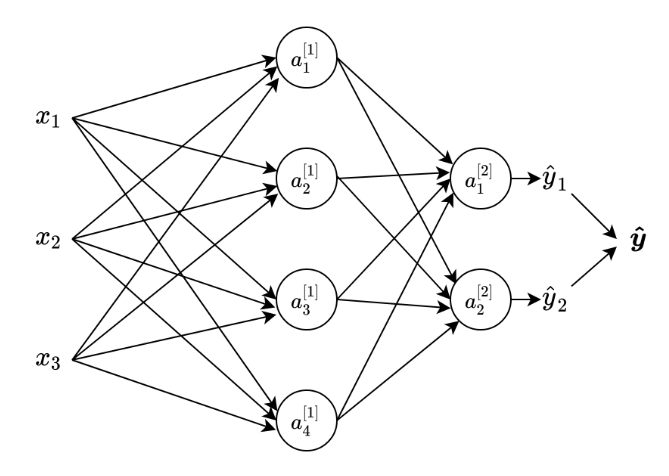
\includegraphics[width=.7\textwidth]{IMAGES/opti/Screenshot from 2023-11-20 22-44-45.png}
\end{figure}

They are "fully-connected" layers as each neuron (circle) of a layer is connected to all neurons of the following layer. The number of hidden layer corresponds to the depth. Each connection is a weight. After each neuron, we get a non-linear output.\\

Inside a neuron, we have : \begin{itemize}
    \item $x_i$ inputs\\
    \item compute $z = w^Tx+b$\\
    \item then we use the activation function that makes everything non-linear : $a = g(z)$\\
    \item output $a$\\
\end{itemize} 

We use the following representation : $a_i^{[l]}$, l the layer and i the node in layer\\
As well as : $w_i^{[l]}$ the weight vector for node i at layer l\\

We can also write the weight matrix that combines all weight vectors of a layer : $W^{[l]} = \begin{pmatrix}
    w_1^{[l]} & \dots & w_d^{[l]}\\
\end{pmatrix}$ and the biases vector : $b^{[l]} = \begin{pmatrix}
    b_1^{[l]}\\ \vdots \\ b_d\\
\end{pmatrix}$

Therefore, we have $z^{[l]} = W^{[l]T}x+ b^{[l]}$ and after the activation : $a^{[l]}= g^{[l]}(z^{[l]})$\\

\subsubsection{Activation functions}

With two layers, we get that the output is : \begin{equation}
    \hat{y} = g^{[2]} ( W^{[2]T} g^{[1]}(W^{[1]T}x+b^{[1]}) + b^{[2]})
\end{equation}

\footnote{If we remove the activation, we simply end up with a linear classifier.}

Three main types of activation functions : \begin{itemize}
    \item Sigmoid : $f(x) = \frac{1}{1+e^{-x}}$, the output is in [0,1] range and nullifies the gradient, rarely used\\
    \item Tanh : $f(x) = \frac{e^x-e^{-x}}{e^x + e^{-x}}$, the output is in [-1,1] range and also nullifies the gradient, rarely used\\
    \item ReLU (rectified linear unit) : $f(x) = \max(0,x)$, easily computed, simple gradient, accelerates convergence of gradient descent, commonly used\\
    \item Leaky ReLU : $f(x) = \max(.1x,x)$\\
\end{itemize}

Derivatives of each can be written as a function of the function itself and is given below : \begin{itemize}
    \item Sigmoid : $\frac{d}{dx}\sigma(x) = \sigma(x) (1-\sigma(x))$\\
    \item Tanh : $\frac{d}{dx} \tanh(x) = 1-\tanh(x)^2$\\
    \item ReLU : $\frac{d}{dx}ReLU(x) = \begin{cases}
        1 & \text{if x>0}\\
        0 & \text{if x<0}\\
    \end{cases}$ We also take the derivative at 0 to be 0 by convention.\\
\end{itemize}

\subsubsection{Training neural networks}
In order to train the neural network, we need a loss function $L(\hat{y},y)$.\\
We simply consider MSE Loss : \begin{equation}
    L(W,b) = \frac{1}{N} \sum_{i=1}^N(\hat{y}^i-y^i)^2
\end{equation}
Where $\hat{y}^i$ is the prediction of neural network on $x^i$ given W and b.\\

For classification although, we use the cross entropy loss.\\

Then, in order to find the best W and b that minimize the loss function, we use the gradient descent : \\
\begin{equation}
\begin{gathered}
    W^{[i]} = W^{[i]} - \alpha \frac{\partial L}{\partial W^{[i]}}\\
    b^{[i]} = b^{[i]} - \alpha \frac{\partial L}{\partial b^{[i]}}\\
    \end{gathered}
\end{equation}

Where $\alpha$ is the learning rate.\\

We can also use the stochastic gradient descent : \\
\begin{equation}
    W^{[i]} = W^{[i]} - \alpha \frac{\partial}{\partial w} (\hat{y}^{n_i}-y^{n_i})^2\lvert_{(W,b)}
\end{equation}
Where $n_i$ is a random index\\

Or even the mini-batch stochastic gradient descent :\\
It basically is a gradient descent mixed with a stochastic one; we get a batch of data and use gradient descent on it.\\

The problem with training is that the loss function is non-convex and may have lots of local minima.\\

\begin{itemize}
    \item Forward pass : compute the output of a neural network for a given input\\
    \item Backward pass : compute derivatives of the network parameters given the output.\\
\end{itemize}

During training, we use both. During interference (predicting on new data) we only use forward pass.\\

\subsection{Convolutional neural network}
The goal here is to be able to handle images with fully connected neural network. Usually, images have a depth of 3 (for the three channels RGB).\\
Therefore, the number of data is heightxwidthx3 which can be a lot.\\

One way to get the information needed is to \textbf{flatten the image}. Although, by doing so, spatial structure gets lost. Also, it doesn't scale well to large images (i.e. a 1024x1024x3 image results in 3 145 728 weights for each neuron of the first hidden layer!)\\


\subsubsection{Convolution with a filter}
Let $x\in \mathbb{R}^d$ be a signal and $w\in\mathbb{R}^{2m+1}$ a filter.\\$z = w*x \Rightarrow z_i = \sum_{j=-m}^{m} w_j x_{i+j}$\\

In order to compute $z$ at the boundaries we have multiple ways : \begin{itemize}
    \item zero padding : extend $\overline{x} = (0,0,x,0,0)$\\
    \item repetition : $\overline{x} = (x_1, x_1, x, x_d, x_d)$\\
    \item ignore the boundary and return $z\in \mathbb{R}^{d-2m}$\\
\end{itemize}

Filters can approximate what happens in neighborhood with a few numbers : \begin{itemize}
    \item average value of signal in a neighborhood : $w = (\frac{1}{3}, \frac{1}{3}, \frac{1}{3})$\\
    \item sharpen the signal : $w = (-1,4,-1)$\\
    \item blur the signal (Gaussian filter) : $w = (e^{-\frac{1}{2\sigma^2}}, e^0, e^{\frac{1}{2\sigma^2}})$\\
    \item approximate derivative of a signal : $w = (-1,0,1)/(2h)$\\
    \item approximate second derivative : $w = (1,-2,1)/h^2$\\
\end{itemize}

Convolution with a filter is a linear function.\\
We can also apply convolutions to : \begin{itemize}
    \item continuous signals $x : \mathbb{R}\rightarrow\mathbb{R}$ such that $z(t) = x*h = \int_{-\infty}^\infty x(\tau) h(t-\tau)d\tau$\\
    \item matrices $M\in \mathbb{R}^{nxn_2}$\\
\end{itemize}

Convolution for matrices works as follow : \\
\begin{enumerate}
    \item Select a sub-matrix from the input matrix that is the size of the filter and apply a dot product\\
    \item Shift the sub-matrix by one on the side and start again. \\
    \item This reduces by much the size of the output.\\
\end{enumerate}

\warning Filters always extend the full depth of the input volume.\\
Taking the convolution between the filter and the image creates an activation map.\\
We could also consider a second filter. Perform same convolution operation with this filter to get a second activation map.\\

Another way is to do : Pooling\\

\subsubsection{Pooling}
Applying a function in a non-overlapping way to a signal. We therefore need to define two hyper-parameters : \begin{itemize}    \item \textbf{Stride S:} or by how much we move the filter on the image \\
    \item \textbf{Spatial extent F:} or the size of the filter\\
\end{itemize}

Convolutional neural networks may include pooling layers to reduce the spatial size of the representation.\\

Height and width shrink quite quickly due to the repeated convolutions. To avoid this, we can add zero-padding.

\subsubsection{Summary}
The convolution layer accepts a volume of size : $C_{in} x H_1 x W_1$.\\
It requires four hyper-parameters : \begin{itemize}
    \item number of filters K\\
    \item spatial extend of filters F\\
    \item Stride S\\
    \item Amount of zero padding P\\
\end{itemize}

It produces a volume of size : $C_{out} x H_2 x W_2$ where : \begin{itemize}
    \item $C_{out} = K$\\
    \item $H_2 = \frac{(H_1-F+2P)}{S}+1$\\
    \item $W_2 = \frac{(W_1-F+2P)}{S}+1$\\
\end{itemize}

There are $FFC_{in}$ weights per filter.\\

\subsection{Decision trees}
We split the data based on the answer to a question.\\
We have : \begin{itemize}
    \item Root node : the first node\\
    \item Internal node : node that still have branches afterwards\\
    \item Leaf node : last node of a branch\\
\end{itemize}

Nodes are checked on a single feature; branches are feature values and leaves indicate prediction of the tree.\\
They are used for both regression and classification.\\

\subsubsection{Regression tree}
To construct the tree, we have to decide which feature to use at which node and what value to use for the split. \\
The loss function is given by : \begin{equation}
    \min L(j,s) = \sum_{ind1} (y^i- \overline{y}_-)^2 + \sum_{ind2} (y^i- \overline{y}_+)^2
\end{equation}

With : \begin{itemize}
    \item j the feature\\
    \item s the value\\
    \item $ind1 = \{$indices such that $x_j^i\leq s \} \subseteq \{1,2,\dots, K\}$\\
    \item $ind2 = \{$indices such that $x_j^i\geq s \} \subseteq \{1,2,\dots, K\}$\\
    \item $\overline{y}_-$ : average y of values for data points with indices $ind1$\\
    \item $\overline{y}_+$ : average y of values for data points with indices $ind2$\\
\end{itemize}

The loss function is non-convex in j and s and the global loss function would tell us which features and what threshold values to use for the entire tree. Therefore, we use solve the optimization node by node (gready).\\

\quad \underline{Stopping criteria :}\\
\begin{itemize}
    \item if number of data points at leaf node becomes too small we stop\\
    \item if loss at given depth $d_1$ is close to loss at depth $d_2 = d_1+1$ then we may stop\\
\end{itemize}

\subsubsection{Classification tree}
We evaluate performance of a given decision tree with a confusion matrix and we measure accuracy and error rate. Although, it is hard to minimize, therefore we use greedy approach : compute it at each leaf.\\

Choose a feature and the split sequentially based on a metric such as Gini impurity : \begin{itemize}
    \item Gini impurity of a leaf : $p_k$ probability of class k in the given leaf \begin{equation}
        \sum_{k=1}^K \sum_{k\neq k'}p_kp_k' = g
    \end{equation}
    \item Gini impurity of a node : weighted sum of given impurity of the two leaves associated, $p_i$ the probability of leaf node i \begin{equation}
        G = \sum p_i g_i
    \end{equation}
\end{itemize}
We then select the smallest G.\\

The inconvenient of decision trees is that it tends to over-fit if it is too deep and doesn't always perform so well.\\

\subsubsection{Random forests}
We can combine multiple models together in order to reduce one type of error without significantly increasing the other.\\

The idea is to take a collection of predictor and combine their results to make a single predictor.\\

Different types : \begin{itemize}
    \item Bagging : train predictors on different samples of the data and combine outputs through voting or averaging\\
    \item Stacking : combine model outputs using a second stage predictor\\
    \item Boosting : train learners on the filtered output of other \\
\end{itemize}

\quad \underline{Bagging (Bootstrap aggregating) :}\\
Suppose we have n classifiers with each an error rate e. Assume each classifier is independent.\\
The probability that the ensemble classifier makes a wrong prediction (majority makes wrong prediction) is : \begin{equation}
    P(wrong) = \sum_{N/2}^N \begin{pmatrix}
        N\\ i\\
    \end{pmatrix} e^i(1-e)^{N-i}
\end{equation}

\quad \underline{Randomization to reduce correlation :}\\
Two randomization strategies are used to select the data on which the classifier is trained : \begin{itemize}
    \item sampling data : each tree is trained on different data\\
    \item sampling features : corresponding nodes in different trees don't use the same feature to split\\
\end{itemize}

Construction : \begin{enumerate}
    \item Draw K bootstrap samples of size n from the original dataset with replacement\\
    \item while constructing the decision tree, select a random set of m features out of the p features available to infer split\\
\end{enumerate}

\textbf{Prediction as average for regression}.\\
\textbf{Prediction as majority vote for classification}.\\

\subsection{Reinforcement Learning}

It is a type of machine learning in which an agent learns to interact with its environment in order to maximize a reward signal.\\

A \textbf{Markov decision process} is given by : $\mathcal{M} = (\mathcal{S}, \mathcal{A}, P,\rho)$ where : \begin{itemize}
    \item $\mathcal{S}$ : the set of all possible states\\
    \item $\mathcal{A}$ : the set of all possible actions\\
    \item P : the transition law\\
    \item $\rho$ : the initial state distribution $\rho(s) = P(s_0=s)$\\
\end{itemize}

Markov property : \begin{equation}
    P(s_{t+1} \lvert s_t, s_{t-1}, \dots, s_0, a_t, \dots, a_0) = P(s_{t+1} \lvert s_t,a_t)
\end{equation}

\quad \underline{Decision rule :}\\
In state $s\in \mathcal{S}$, we take action $a\in \mathcal{A}$ with probability $\pi(a\lvert s)$\\

\quad \underline{Reward and discount factor :}\\
Reward function $r: \mathcal{S}x\mathcal{A} \rightarrow \mathbb{R}$\\
Discount rate $\gamma \in (0,1)$\\

The goal is to find an optimal policy $\pi^*$ maximizing : \begin{equation}
    J(\pi) = \mathbb{E} [\sum_{t=0}^\infty \gamma^t r(s_t,a_t)\lvert s_0, \rho, \pi]
\end{equation}

We here use the policy gradient method : \\
parameterize the policy as $\pi_\theta(a\lvert s)$ and then find the best policy.\\

\begin{itemize}
    \item Direct parametrization : $\pi_\theta(a\lvert s) = \theta_{s,a}$ where $\theta \in \mathbb{R}^{\mathcal{S}x \mathcal{A}}$, $\theta_{s,a} \geq 0$ and $\sum \theta_{s,a} = 1$\\
    \item Softmax : $\pi_\theta (a\lvert s) = \frac{e^{\theta_{s,a}}}{\sum_{a'\in \mathcal{A}} e^{\theta_{s,a'}}}$\\
    \item Neural softmax : $\pi_\theta(a\lvert s) = \frac{e^{f_{\theta_{s,a}}}}{\sum_{a'\in \mathcal{A}} e^{f_{\theta_{s,a'}}}}$, where $f_\theta$ represents a neural network.\\
\end{itemize}

We then use the gradient method in order to find the best $\theta$ such that at each iteration : $\theta = \theta + \alpha \nabla_\theta J(\pi_\theta)$\\

Convergence for the different parametrization : let $\rho(s) >0$, $\forall s \in \mathcal{S}$,\\ \begin{itemize}
    \item Direct : $\alpha \leq \frac{(1-\gamma)^3}{2\gamma \lvert \mathcal{A}\rvert}$, we have $\min J(\pi^*)-J(\pi) \leq \frac{c_1}{\sqrt{K}}$\\
    \item Softmax : $\alpha \leq \frac{(1-\gamma)^3}{8}$, we have $\min J(\pi^*)-J(\pi) \leq \frac{c_2}{K}$\\
\end{itemize}
Where $c_1$ and $c_2$ are the constant that depend on MDP.\\

For every random trajectory $\tau$, the probability of choosing this trajectory is : $p_\theta(\tau) = \rho(s_0) \Pi_{t=0}^\infty \pi_\theta(a_t\lvert s_t) P(s_{t+1}\lvert s_t,a_t)$.\\

The reward we get from this trajectory : $R(\tau) = \sum_{t=0}^\infty \gamma^t r(s_t,a_t)$\\

Then : \begin{equation} \begin{gathered}
    J(\pi_\theta) = \mathbb{E}_{\tau, p_\theta} [R(\tau)]\\
    \nabla_\theta J(\pi_\theta) = \sum_{t=0}^\infty \gamma^tr(s_t,a_t)\\
    = \frac{1}{N} \sum_{i=1}^N (\sum_{t=0}^H \gamma^t r(s_t^i, a_t^i)) (\sum_{t=0}^H \nabla_\theta \log \pi_\theta(a_t,s_t))\\
    \end{gathered}
\end{equation}

\quad \underline{Stochastic policy gradient method :}\\
For i from 1 to number of trajectory, generate a trajectory and compute its policy gradient estimator.\\
Then return policy gradient estimator : $\hat{\nabla}_\theta J(\pi_\theta) = \frac{1}{N} \sum_{i=1}^N \nabla_i J(\pi_\theta)$\\

\begin{itemize}
    \item Pros : \begin{itemize}
        \item General methods for complex tasks\\
        \item Adapt to changing environments\\
    \end{itemize}
    \item Cons : \begin{itemize}
        \item Sample inefficiency for model free approach\\
        \item Lack of safety and convergence\\
    \end{itemize}
\end{itemize}







\end{document}